
%(BEGIN_QUESTION)
% Copyright 2010, Tony R. Kuphaldt, released under the Creative Commons Attribution License (v 1.0)
% This means you may do almost anything with this work of mine, so long as you give me proper credit

This flowmeter (Annubar flow element, Yokogawa DP transmitter) is used to measure the flow of air through a large pipe.  The installation could be improved, though:

$$\epsfxsize=5in \includegraphics[width=15.5cm]{i01400x01.eps}$$

Explain how you would improve this flowmeter installation if you were tasked with re-doing it.

\underbar{file i01400}
%(END_QUESTION)





%(BEGIN_ANSWER)

Being and air (gas) process, the DP transmitter should be mounted {\it above} the flow element, not below.  As it is built, a technician must periodically open the vent valves (located at the bottom ``tee'' fittings on the impulse lines) to drain any accumulated liquid.

%(END_ANSWER)





%(BEGIN_NOTES)

{\bf This question is intended for exams only and not worksheets!}.

%(END_NOTES)

